% L10c lecture companion. Notebook hashes and coverage are recorded in README.md.
% Style files and Cornell seal are copied unchanged from the L10a deck (identical
% to L9c and L9a, which match the approved L6a deck). The bandit arms and UCB
% example figures are the light PDFs from ../figs, copied into assets/ by
% `make figures`.
%
% Notation follows the lecture: arms a in A with |A| = K, rounds t = 1, ..., T,
% reward distributions D_a, mean rewards mu(a), the best mean mu^star, gaps
% Delta(a), regret R(T), cumulative gap loss G(T), sample means \bar{mu}(a),
% pull counts N_a, exploration probability epsilon_t, confidence radius U(a,t),
% Bernoulli success probabilities theta_a, Beta parameters alpha(a), beta(a),
% successes S(a), failures F(a), and posterior samples p(a). log is natural.
\documentclass[aspectratio=169,11pt]{beamer}
\usepackage{vnslides}
\renewcommand{\vnlecturecode}{L10c}
\newcommand{\lecturelink}{https://github.com/varnerlab/CHEME-5800-CourseRepository-Fall-2026/blob/main/weeks/week-10/L10c/CHEME-5800-L10c-Lecture-StochasticMultiarmBandits-Fall-2026.ipynb}
\newcommand{\lablink}{https://github.com/varnerlab/CHEME-5800-CourseRepository-Fall-2026/blob/main/weeks/week-10/L10d/CHEME-5800-L10d-Lab-BanditAlgorithms-Fall-2026.ipynb}
\newcommand{\slivkinslink}{https://arxiv.org/abs/1904.07272}
\newcommand{\lecturesource}[1]{\note{[Sources]\par
  \href{\lecturelink}{L10c lecture: Stochastic Multi-Armed Bandit Problems.}\par
  #1\par[/Sources]}}
\newcommand{\A}{\mathcal A}
\newcommand{\mub}{\bar{\mu}}
\newcommand{\BetaDist}{\operatorname{Beta}}

\title{\texorpdfstring{{\vnheavy L10c}}{L10c}: Stochastic Multi-Armed Bandits}
\subtitle{\texorpdfstring{Exploration, regret, UCB1, and Thompson sampling\\[3pt]CHEME 5800 Cornell University}{Exploration, regret, UCB1, and Thompson sampling; CHEME 5800 Cornell University}}
\author{Copyright Jeffrey Varner 2026. All Rights Reserved}

\begin{document}
\special{pdf:minorversion 7}
\vntitlepage

\begin{frame}{Objectives for Today}
  How should an agent choose among actions with unknown rewards, when it sees
  only the reward of the action it takes?

  \vspace{0.4em}
  {\large\textbf{\ink{Today's concepts}}}
  \vspace{0.2em}
  \begin{itemize}\setlength{\itemsep}{0.4em}
    \item \hilite{Balance exploration and exploitation}: choose between trying
      actions to learn about them and taking the action that looks best so far,
      and see why an agent needs both.
    \item \hilite{Solve multi-armed bandit problems}: choose the next arm with
      the explore-first, epsilon-greedy, UCB1, and Thompson sampling
      algorithms.
    \item \hilite{Compare bandit algorithms with regret}: define the regret of
      a bandit algorithm and compare the expected-regret bounds of
      explore-first, epsilon-greedy, and UCB1.
  \end{itemize}
  \slidenote{Lecture:}{\href{\lecturelink}{Stochastic Multi-Armed Bandit Problems}}
  \lecturesource{Introduction and three Learning Objectives.}
\end{frame}

\begin{frame}{Exploration vs. Exploitation}
  An agent chooses an action, receives a reward, and uses that observation to
  decide what to try next. Its goal is to collect as much reward as possible.

  \vspace{0.6em}
  \begin{itemize}\setlength{\itemsep}{0.7em}
    \item \hilite{Exploration}: try actions that have not been tried often, to
      learn about their rewards.
    \item \hilite{Exploitation}: take the action that looks best so far. An
      agent that only exploits never tries anything new; how boring!
  \end{itemize}

  \vspace{0.8em}
  Explore too much, and we give up reward now. Exploit too much, and we may
  write off an action whose low observed reward was simply bad luck.
  \lecturesource{Exploration vs. Exploitation: opening paragraph, the two numbered items, and the closing paragraph.}
\end{frame}

\begin{frame}{What Is a Bandit Problem?}
  An agent repeatedly chooses among $K$ options, called \hilite{arms}, and
  receives a reward from the arm it pulls.

  \vspace{0.2em}
  \centering
  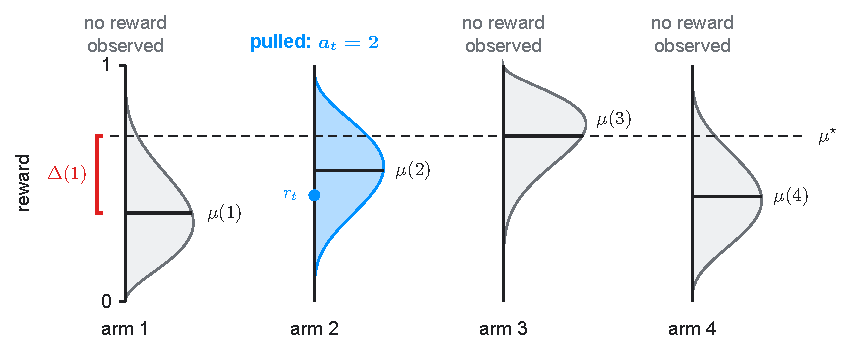
\includegraphics[width=\textwidth,height=0.48\paperheight,keepaspectratio]{assets/Fig-Bandit-Arms.pdf}

  \vspace{0.2em}
  \raggedright
  \hilite{Only the pulled arm reports a reward.} In round $t$, arm $a_t$ yields
  reward $r_t$; $\mu^\star$ is the largest of the unseen means $\mu(a)$, and
  $\Delta(1)$ is arm 1's gap below it.
  \lecturesource{What Is a Bandit Problem?: definition, figure, and caption.
    Figure: ../figs/Fig-Bandit-Arms (TikZ, light PDF).}
\end{frame}

\begin{frame}{Bandit Problems in Practice}
  Each system tries one option at a time and sees only that option's outcome:

  \vspace{0.4em}
  \centering
  {\small\setlength{\tabcolsep}{4pt}%
  \begin{tabular}{>{\raggedright\arraybackslash}p{0.22\textwidth}>{\raggedright\arraybackslash}p{0.21\textwidth}>{\raggedright\arraybackslash}p{0.24\textwidth}>{\raggedright\arraybackslash}p{0.24\textwidth}}
    \toprule
    \textbf{Application} & \textbf{Arms} & \textbf{Reward of one pull} & \textbf{Cost of exploring}\\
    \midrule
    Clinical trials\newline{\scriptsize\href{https://pmc.ncbi.nlm.nih.gov/articles/PMC4856206/}{Villar et al., 2015}} & treatments given to patients & 1 if the treatment works, 0 if not & some patients get a less effective treatment\\
    \addlinespace[2pt]
    News recommendation\newline{\scriptsize\href{https://arxiv.org/abs/1003.0146}{Li et al., 2010}} & articles for the Yahoo!\ front page & 1 if the visitor clicks, 0 if not & some visitors see a less popular article\\
    \addlinespace[2pt]
    Network routing\newline{\scriptsize\href{https://arxiv.org/abs/1309.7367}{Talebi et al., 2018}} & paths through a computer network & time for the data to arrive & some data take a slower path\\
    \addlinespace[2pt]
    Online pricing\newline{\scriptsize\href{https://doi.org/10.1287/mksc.2018.1129}{Misra et al., 2019}} & candidate prices for a product & profit on the sale, 0 if no sale & some customers see a less profitable price\\
    \bottomrule
  \end{tabular}}

  \vspace{0.4em}
  \raggedright
  Delay and profit are rescaled to $[0,1]$, with faster or more profitable
  closer to 1.
  \lecturesource{What Is a Bandit Problem?: applications table and the rescaling sentence.
    The lead sentence and the table's cells are shortened from the lecture's.}
\end{frame}

\begin{frame}{Stochastic Bandit Model}
  The agent has a fixed set of arms $\A$, with $|\A|=K$, and plays for $T$
  rounds. Arm $a$ draws its rewards from a distribution $\mathcal D_a$ on
  $[0,1]$, with mean reward $\mu(a)=\mathbb E_{r\sim\mathcal D_a}[r]$.

  \vspace{0.4em}
  For $t=1,2,\ldots,T$ \textbf{do}:
  \begin{enumerate}\setlength{\itemsep}{0.2em}
    \item The agent chooses an arm $a_t\in\A$ using its previous actions and
      observed rewards.
    \item The environment independently draws $r_t\sim\mathcal D_{a_t}$.
    \item The agent receives $r_t$ and updates its estimates.
  \end{enumerate}

  \vspace{0.5em}
  The regret bounds assume independent draws, \hilite{stationary}
  distributions (they do not change), and rewards between 0 and 1. Maximizing
  total reward is the same goal as minimizing \hilite{regret}.
  \lecturesource{Stochastic Bandit Model: definition, assumptions, the For loop, and the goal paragraph.}
\end{frame}

\begin{frame}{Regret}
  Let $\mu^\star=\max_{a\in\A}\mu(a)$. Always pulling the best arm earns
  $T\mu^\star$ in expectation, so the regret of one game (one run of $T$
  rounds) and the \hilite{cumulative gap loss} are:
  \[
    R(T)=T\mu^\star-\sum_{t=1}^{T}r_t,
    \qquad
    G(T)=\sum_{t=1}^{T}\Delta(a_t),\quad\Delta(a)=\mu^\star-\mu(a).
  \]

  \vspace{0.2em}
  \begin{itemize}\setlength{\itemsep}{0.4em}
    \item $R(T)$ moves with reward luck, even after the agent has found the
      best arm.
    \item $G(T)$ adds the mean reward given up by each pull, so a pull of the
      best arm adds nothing.
  \end{itemize}

  \vspace{0.3em}
  A pull of $a_t$ has expected reward $\mu(a_t)$, so the two agree on average:
  \[
    \boxed{\mathbb E[R(T)]=\mathbb E[G(T)]}
  \]
  \lecturesource{Regret: R(T), the gap loss G(T) (pseudo-regret), and the expectation identity.}
\end{frame}

\begin{frame}{Explore-First Algorithm}
  Pull each arm $N$ times (exploration), then pull the arm with the highest
  sample mean for the rest of the game (exploitation).

  \vspace{0.4em}
  \textbf{Initialize}: Given $K$ arms and the number of rounds $T\ge K$, choose
  \[
    N=\min\left\{\left\lfloor\frac{T}{K}\right\rfloor,\;\max\left\{1,\;\operatorname{round}\left[\left(\frac{T}{K}\right)^{2/3}(\log T)^{1/3}\right]\right\}\right\}.
  \]
  \begin{enumerate}\setlength{\itemsep}{0.2em}
    \item For each arm $a\in\A$ \textbf{do}: pull arm $a$ for $N$ rounds and
      compute its sample mean $\mub(a)$, the average of its $N$ rewards.
    \item Choose $\hat a\gets\arg\max_{a\in\A}\mub(a)$, breaking ties by the
      first arm index.
    \item For $t=KN+1,\ldots,T$ \textbf{do}: pull arm $\hat a$.
  \end{enumerate}

  \vspace{0.3em}
  Here, $\log$ is the natural logarithm; the $\max$ pulls every arm at least
  once, and the $\min$ fits the exploration in $T$ rounds.
  \lecturesource{Explore-First Exploration: description and Explore-First Algorithm. Preserve the Initialize/For/numbered-step format.}
\end{frame}

\begin{frame}{Explore-First: Regret Bound}
  With $N$ of order $(T/K)^{2/3}(\log T)^{1/3}$, explore-first achieves
  \href{\slivkinslink}{(Slivkins, Theorem 1.5)}:
  \[
    \boxed{\mathbb E[R(T)]\le T^{2/3}\cdot\mathcal O(K\log T)^{1/3}}
  \]
  This $N$ balances the cost of
  exploring against the cost of committing to a poorly estimated arm.

  \vspace{0.8em}
  \begin{itemize}\setlength{\itemsep}{0.5em}
    \item \hilite{Of order $x$}: a constant multiple of $x$.
    \item \hilite{Big-O}, $\mathcal O(x)$: at most a constant multiple of $x$.
  \end{itemize}
  Neither constant depends on $T$ or $K$.
  \lecturesource{Explore-First Exploration: Theorem, the balance sentence, and the order and big-O paragraph.}
\end{frame}

\begin{frame}{Epsilon-Greedy Algorithm}
  Spread exploration out: pull a random arm with probability $\epsilon_t$,
  which shrinks over time, and the best arm so far otherwise.

  \vspace{0.3em}
  \textbf{Initialize}: Given $K$ arms and $T\ge K$ rounds, pull each arm once and
  call its reward $r_a$; set its pull count $N_a\gets1$ and sample mean
  $\mub(a)\gets r_a$.

  \vspace{0.2em}
  For $t=K+1,\ldots,T$ \textbf{do}:
  \begin{enumerate}\setlength{\itemsep}{0.15em}
    \item Draw $u$ uniformly from $[0,1]$ and compute
      $\epsilon_t=\min\left\{1,\left(K\log t/t\right)^{1/3}\right\}$.
    \item Choose the arm $a_t$:
      \begin{itemize}\setlength{\itemsep}{0.1em}
        \item If $u\le\epsilon_t$ \textbf{then} choose $a_t\in\A$ uniformly at
          random (exploration).
        \item Otherwise, $a_t\gets\arg\max_{a\in\A}\mub(a)$, breaking ties by
          the first arm index (exploitation).
      \end{itemize}
    \item Pull arm $a_t$ and receive a reward $r_t$ from the environment.
    \item Update the pull count $N_{a_t}$ and the sample mean $\mub(a_t)$.
  \end{enumerate}
  \lecturesource{Epsilon-Greedy Exploration: idea and Epsilon-Greedy Algorithm (its Theorem is on the Comparing the Regret Bounds slide). Preserve the Initialize/For/numbered-step format and the If/Otherwise branches.}
\end{frame}

\begin{frame}{Optimism Under Uncertainty}
  Assume each arm is as good as it can be given the observations so far, and
  pull the arm with the best optimistic estimate.

  \vspace{0.5em}
  The \hilite{upper confidence bound} of arm $a$ at round $t$ is
  $\mub(a)+U(a,t)$, where the \hilite{confidence radius} is an allowance for how
  uncertain the sample mean still is:
  \[
    U(a,t)=\sqrt{\frac{2\log t}{N_a}},
  \]
  and $N_a$ is the number of times arm $a$ has been pulled before round $t$.

  \vspace{0.5em}
  With high probability, the upper confidence bound lies above the true mean
  $\mu(a)$. This idea leads to the UCB1 algorithm of
  \href{https://doi.org/10.1023/A:1013689704352}{Auer, Cesa-Bianchi, and Fischer (2002)}.
  \lecturesource{Optimism Under Uncertainty: opening paragraph and the UCB definition.}
\end{frame}

\begin{frame}{UCB1 Algorithm}
  \textbf{Initialize}: Given $K$ arms and $T\ge K$ rounds, pull each arm once and
  call its reward $r_a$; set its pull count $N_a\gets1$ and sample mean
  $\mub(a)\gets r_a$.

  \vspace{0.3em}
  For $t=K+1,\ldots,T$ \textbf{do}:
  \begin{enumerate}\setlength{\itemsep}{0.25em}
    \item Compute the confidence radius $U(a,t)$ for each arm $a\in\A$.
    \item Choose the arm with the largest upper confidence bound,
      $a_t\gets\arg\max_{a\in\A}\left\{\mub(a)+U(a,t)\right\}$, breaking ties
      by the first arm index.
    \item Pull arm $a_t$ and receive a reward $r_t$ from the environment.
    \item Update the pull count $N_{a_t}$ and the sample mean $\mub(a_t)$.
  \end{enumerate}

  \vspace{0.6em}
  UCB1 achieves \href{\slivkinslink}{(Slivkins, Theorem 1.15)}:
  \[
    \boxed{\mathbb E[R(T)]\le\mathcal O\left(\sqrt{KT\log T}\right)}
  \]
  \lecturesource{Optimism Under Uncertainty: UCB1 Algorithm and Theorem. Preserve the Initialize/For/numbered-step format.}
\end{frame}

\begin{frame}{Worked Example: Two Arms, Five Rounds}
  After five rounds, arm 1 has four pulls with $\mub(1)=0.75$, and arm 2 has
  one pull with $\mub(2)=0$. Before round $t=6$:

  \vspace{0.2em}
  \centering
  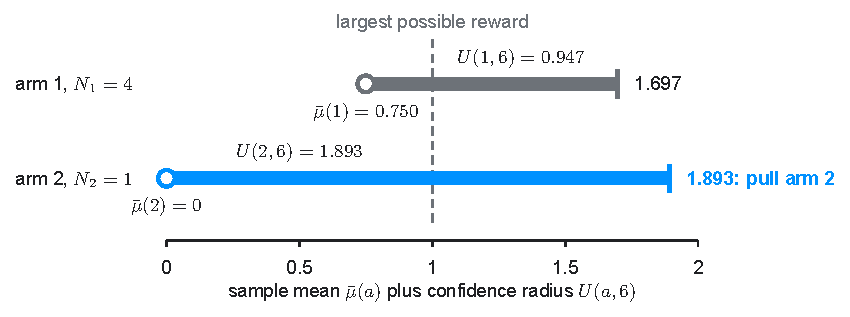
\includegraphics[width=\textwidth,height=0.45\paperheight,keepaspectratio]{assets/Fig-UCB-Example.pdf}

  \vspace{0.2em}
  \raggedright
  \hilite{One observation leaves more uncertainty than four.} UCB1 pulls arm 2,
  whose bound $1.893$ beats arm 1's $1.697$, even above the largest possible
  reward of 1.
  \lecturesource{Optimism Under Uncertainty: Worked Example, figure, and caption.
    Figure: ../figs/Fig-UCB-Example (TikZ, light PDF).}
\end{frame}

\begin{frame}{Comparing the Regret Bounds}
  \centering
  {\small\setlength{\tabcolsep}{6pt}%
  \begin{tabular}{>{\raggedright\arraybackslash}p{0.18\textwidth}>{\raggedright\arraybackslash}p{0.42\textwidth}>{\raggedright\arraybackslash}p{0.26\textwidth}}
    \toprule
    \textbf{Algorithm} & \textbf{How it explores} & \textbf{Expected-regret bound}\\
    \midrule
    Explore-first & pulls every arm $N$ times, then commits to one arm & $T^{2/3}\cdot\mathcal O(K\log T)^{1/3}$\\
    \addlinespace
    Epsilon-greedy & pulls a random arm with probability $\epsilon_t$, which shrinks over time & $T^{2/3}\cdot\mathcal O(K\log T)^{1/3}$\\
    \addlinespace
    UCB1 & pulls the arm with the largest upper confidence bound & $\mathcal O\left(\sqrt{KT\log T}\right)$\\
    \bottomrule
  \end{tabular}}

  \vspace{0.5em}
  \raggedright
  All three grow more slowly than $T$, so the expected regret per round shrinks
  toward zero as the game gets longer. The UCB1 bound grows with about
  $\sqrt T$ rather than $T^{2/3}$, the strongest guarantee of the three.

  \vspace{0.3em}
  {\small Bounds from \href{\slivkinslink}{Slivkins}, Theorems 1.5, 1.6, and
  1.15. The epsilon-greedy bound, with the capped $\epsilon_t$, holds at every
  round $t$.}
  \lecturesource{Comparing the Regret Bounds: table and closing paragraph; the epsilon-greedy Theorem from Epsilon-Greedy Exploration.}
\end{frame}

\begin{frame}{Binary Bernoulli Bandit Problem}
  Each reward is binary, $r_t\in\{0,1\}$: arm $a$ pays 1 with an unknown
  probability $\theta_a$, so $r\sim\texttt{Bern}(\theta_a)$ and
  $\mu(a)=\theta_a$.

  \vspace{0.5em}
  Ready to get your mind blown? We can represent our uncertainty about each
  $\theta_a$ with a \hilite{prior}, our belief before any rewards, and update
  it as rewards arrive:
  \begin{itemize}\setlength{\itemsep}{0.4em}
    \item $\BetaDist(\alpha,\beta)$ describes an unknown probability on $[0,1]$;
      $\alpha,\beta>0$ set its shape, its mean is $\alpha/(\alpha+\beta)$, and
      $\BetaDist(1,1)$ is uniform.
    \item After $S$ successes and $F$ failures, the \hilite{posterior}, our
      updated belief, is again a Beta distribution:
  \end{itemize}
  \[
    \boxed{\BetaDist(\alpha,\beta)\;\longrightarrow\;\BetaDist(\alpha+S,\,\beta+F)}
  \]
  \lecturesource{Binary Bernoulli Bandit Problem: the model, the "Ready to get your mind blown?" paragraph, and the Beta distribution box.}
\end{frame}

\begin{frame}{Epsilon-Greedy for the Bernoulli Bandit}
  The epsilon-greedy algorithm carries over with two changes:
  \begin{enumerate}\setlength{\itemsep}{0.4em}
    \item Track the successes $S(a)$ and failures $F(a)$ of each arm, starting
      from $S(a)=F(a)=0$ and uniform priors, $\alpha(a)=\beta(a)=1$.
    \item When exploiting, pull the arm with the highest \hilite{posterior
      mean}:
      \[
        a_t\gets\arg\max_{a\in\A}\left\{\frac{\alpha(a)+S(a)}{\alpha(a)+\beta(a)+S(a)+F(a)}\right\}.
      \]
  \end{enumerate}
  After each pull, update the counts of the arm we pulled:
  \[
    S(a_t)\gets S(a_t)+r_t,\qquad F(a_t)\gets F(a_t)+(1-r_t).
  \]
  Everything else is unchanged: pull each arm once, then explore at random
  with probability $\epsilon_t$.
  \lecturesource{epsilon-Greedy Binary Bernoulli Bandit: the two changes, the posterior-mean rule, and the count update.}
\end{frame}

\begin{frame}{Thompson Sampling Algorithm}
  \textbf{Initialize}: Given $K$ arms and $T\ge1$ rounds, set
  $\alpha(a)\gets1$, $\beta(a)\gets1$, $S(a)\gets0$, and $F(a)\gets0$ for each
  arm $a\in\A$.

  \vspace{0.3em}
  For $t=1,2,\ldots,T$ \textbf{do}:
  \begin{enumerate}\setlength{\itemsep}{0.25em}
    \item Sample $p(a)\sim\BetaDist\left(\alpha(a)+S(a),\,\beta(a)+F(a)\right)$
      for every arm $a\in\A$.
    \item Choose the arm with the highest sample,
      $a_t\gets\arg\max_{a\in\A}\{p(a)\}$.
    \item Pull arm $a_t$ and receive $r_t\in\{0,1\}$ from the environment.
    \item Update $S(a_t)\gets S(a_t)+r_t$ and $F(a_t)\gets F(a_t)+(1-r_t)$.
  \end{enumerate}

  \vspace{0.5em}
  Thompson sampling explores mostly arms that could still be the best, so it
  often beats epsilon-greedy \href{https://arxiv.org/abs/1707.02038}{(Russo et
  al., 2020)}. \href{https://doi.org/10.1093/biomet/25.3-4.285}{Thompson
  (1933)} proposed it for two treatments: give each one with the probability
  that it is the better one.
  \lecturesource{Thompson Sampling Binary Bernoulli Bandit: Thompson Sampling Algorithm and the paragraph after it. The Thompson (1933) line is from the What Is a Bandit Problem? section.}
\end{frame}

\begin{frame}{Worked Example: Updating a Bernoulli Arm}
  Uniform $\BetaDist(1,1)$ priors; arm 1 has 3 successes and 1 failure, arm 2
  has 1 failure.

  \vspace{0.2em}
  \centering
  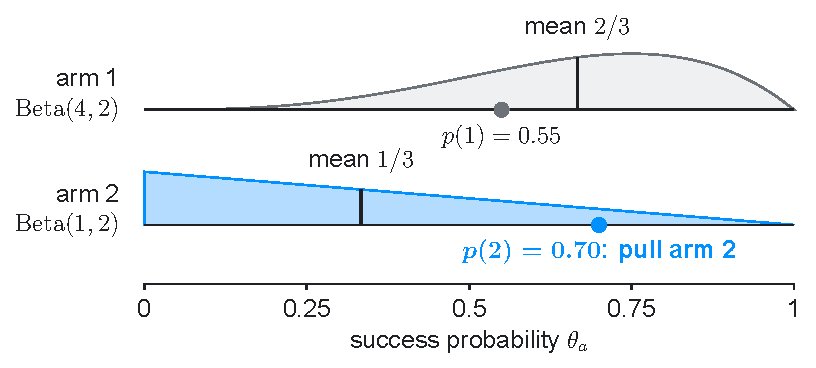
\includegraphics[width=\textwidth,height=0.52\paperheight,keepaspectratio]{assets/Fig-Thompson-Example.pdf}

  \vspace{0.2em}
  \raggedright
  \hilite{Sampling gives an uncertain arm another trial.} Arm 2's sample wins,
  so it is pulled; a success makes its posterior $\BetaDist(2,2)$, mean $1/2$.
  \lecturesource{Thompson Sampling Binary Bernoulli Bandit: the Worked Example.
    Figure: ../figs/Fig-Thompson-Example (TikZ, light PDF); drawn for the deck.}
\end{frame}

\begin{frame}{Lab: Bandit Algorithms}
  In the \href{\lablink}{lab}, we put these algorithms to work:

  \vspace{0.6em}
  \begin{itemize}\setlength{\itemsep}{0.6em}
    \item we run \hilite{explore-first}, \hilite{epsilon-greedy}, and
      \hilite{UCB1} on a bandit with seven arms and compare their regret with
      the bounds,
    \item we implement \hilite{Thompson sampling} for a binary Bernoulli bandit
      and watch the posterior of the best arm concentrate around its true
      success probability, while the arms it rarely pulls stay uncertain.
  \end{itemize}
  \slidenote{Lab:}{\href{\lablink}{Bandit algorithms}}
  \lecturesource{Lab section. Lab notebook: introduction and Learning Objectives.}
\end{frame}

\begin{frame}{Summary}
  We introduced the stochastic multi-armed bandit problem and four algorithms
  for balancing exploration and exploitation.

  \vspace{0.5em}
  {\large\textbf{\ink{Key takeaways}}}
  \vspace{0.3em}
  \begin{itemize}\setlength{\itemsep}{0.6em}
    \item \textbf{\ink{Exploration and exploitation.}} Too little exploration can
      lock an agent onto an arm that only looked good by chance.
    \item \textbf{\ink{Bandit algorithms.}} Four ways to explore: up front, at
      random, optimistically, or by sampling posteriors.
    \item \textbf{\ink{Regret bounds.}} The UCB1 bound grows with about
      $\sqrt T$; the explore-first and epsilon-greedy bounds, with $T^{2/3}$.
  \end{itemize}

  \vspace{0.5em}
  When actions also change the state of the environment, we use a Markov
  decision process.
  \lecturesource{Summary: three key takeaways and concluding sentence.}
\end{frame}

\end{document}
